% Options for packages loaded elsewhere
\PassOptionsToPackage{unicode}{hyperref}
\PassOptionsToPackage{hyphens}{url}
%
\documentclass[
  a4paper,
]{article}
\usepackage{amsmath,amssymb}
\usepackage{setspace}
\usepackage{iftex}
\ifPDFTeX
  \usepackage[T1]{fontenc}
  \usepackage[utf8]{inputenc}
  \usepackage{textcomp} % provide euro and other symbols
\else % if luatex or xetex
  \usepackage{unicode-math} % this also loads fontspec
  \defaultfontfeatures{Scale=MatchLowercase}
  \defaultfontfeatures[\rmfamily]{Ligatures=TeX,Scale=1}
\fi
\usepackage{lmodern}
\ifPDFTeX\else
  % xetex/luatex font selection
\fi
% Use upquote if available, for straight quotes in verbatim environments
\IfFileExists{upquote.sty}{\usepackage{upquote}}{}
\IfFileExists{microtype.sty}{% use microtype if available
  \usepackage[]{microtype}
  \UseMicrotypeSet[protrusion]{basicmath} % disable protrusion for tt fonts
}{}
\makeatletter
\@ifundefined{KOMAClassName}{% if non-KOMA class
  \IfFileExists{parskip.sty}{%
    \usepackage{parskip}
  }{% else
    \setlength{\parindent}{0pt}
    \setlength{\parskip}{6pt plus 2pt minus 1pt}}
}{% if KOMA class
  \KOMAoptions{parskip=half}}
\makeatother
\usepackage{xcolor}
\usepackage[margin=1in]{geometry}
\usepackage{longtable,booktabs,array}
\usepackage{calc} % for calculating minipage widths
% Correct order of tables after \paragraph or \subparagraph
\usepackage{etoolbox}
\makeatletter
\patchcmd\longtable{\par}{\if@noskipsec\mbox{}\fi\par}{}{}
\makeatother
% Allow footnotes in longtable head/foot
\IfFileExists{footnotehyper.sty}{\usepackage{footnotehyper}}{\usepackage{footnote}}
\makesavenoteenv{longtable}
\usepackage{graphicx}
\makeatletter
\def\maxwidth{\ifdim\Gin@nat@width>\linewidth\linewidth\else\Gin@nat@width\fi}
\def\maxheight{\ifdim\Gin@nat@height>\textheight\textheight\else\Gin@nat@height\fi}
\makeatother
% Scale images if necessary, so that they will not overflow the page
% margins by default, and it is still possible to overwrite the defaults
% using explicit options in \includegraphics[width, height, ...]{}
\setkeys{Gin}{width=\maxwidth,height=\maxheight,keepaspectratio}
% Set default figure placement to htbp
\makeatletter
\def\fps@figure{htbp}
\makeatother
\setlength{\emergencystretch}{3em} % prevent overfull lines
\providecommand{\tightlist}{%
  \setlength{\itemsep}{0pt}\setlength{\parskip}{0pt}}
\setcounter{secnumdepth}{-\maxdimen} % remove section numbering
\ifLuaTeX
\usepackage[bidi=basic]{babel}
\else
\usepackage[bidi=default]{babel}
\fi
\babelprovide[main,import]{catalan}
% get rid of language-specific shorthands (see #6817):
\let\LanguageShortHands\languageshorthands
\def\languageshorthands#1{}
\ifLuaTeX
  \usepackage{selnolig}  % disable illegal ligatures
\fi
\usepackage{bookmark}
\IfFileExists{xurl.sty}{\usepackage{xurl}}{} % add URL line breaks if available
\urlstyle{same}
\hypersetup{
  pdfauthor={@tofermos 2024},
  pdflang={ca-ES},
  hidelinks,
  pdfcreator={LaTeX via pandoc}}

\title{UD1. Introducció als SOX (II).}
\usepackage{etoolbox}
\makeatletter
\providecommand{\subtitle}[1]{% add subtitle to \maketitle
  \apptocmd{\@title}{\par {\large #1 \par}}{}{}
}
\makeatother
\subtitle{Configuració bàsica de xarxa en Windows i VirtualBox}
\author{@tofermos 2024}
\date{}

\begin{document}
\maketitle

{
\setcounter{tocdepth}{2}
\tableofcontents
}
\setstretch{1.5}
\newpage

\renewcommand\tablename{Tabla}

\section{1 La connexió de la xarxa a nivell físic
(VirtualBox).}\label{la-connexiuxf3-de-la-xarxa-a-nivell-fuxedsic-virtualbox.}

Una vegada instal·lem les MV Windows 11 hem d'assegurar-nos que tinguen
una tarja de xarxa per poder comunicar-se entre elles.

De totes les opcions que ens apareixen anem a centrar-nos en les que més
ens poden interessar.

\begin{itemize}
\item
  \textbf{Adaptador pont} fa que la MV aparega com un PC més de la xarxa
  local real de l'aula o de ta casa. Tindrà una IP del mateix rang que
  la de l'amfitrió si ha sigut porporcionada pel servei del router.
\item
  \textbf{NAT} Assigan una IP de rang (inclús de classe) ditinta a la
  del teu PC amfitrió.
\item
  \textbf{XARXA INTERNA} A l'igual que l'anterior però ens permet
  assignar un \textbf{nom a la xarxa}.
\end{itemize}

Aquesta última opció és la que usarem quasi sempre al curs present. Els
PCs ( clients i servidors) que han d'estar en la mateix xarxa han de
tenir en aquest camp el mateix nom.

\emph{Taula 1. Resum característiques xarxa VirtualBox}

\begin{longtable}[]{@{}
  >{\raggedright\arraybackslash}p{(\columnwidth - 8\tabcolsep) * \real{0.2000}}
  >{\raggedright\arraybackslash}p{(\columnwidth - 8\tabcolsep) * \real{0.2000}}
  >{\raggedright\arraybackslash}p{(\columnwidth - 8\tabcolsep) * \real{0.2000}}
  >{\raggedright\arraybackslash}p{(\columnwidth - 8\tabcolsep) * \real{0.2000}}
  >{\raggedright\arraybackslash}p{(\columnwidth - 8\tabcolsep) * \real{0.2000}}@{}}
\toprule\noalign{}
\begin{minipage}[b]{\linewidth}\raggedright
Té accés a internet
\end{minipage} & \begin{minipage}[b]{\linewidth}\raggedright
Pot comunicar-se amb altres MV
\end{minipage} & \begin{minipage}[b]{\linewidth}\raggedright
Es pot comunicar amb la màquina real
\end{minipage} & \begin{minipage}[b]{\linewidth}\raggedright
Hem de configurar alguna cosa a Linux/Windows
\end{minipage} & \begin{minipage}[b]{\linewidth}\raggedright
\end{minipage} \\
\midrule\noalign{}
\endhead
\bottomrule\noalign{}
\endlastfoot
NAT & Sí & No & No & No \\
XARXA INTERNA & No & Sí & No & Sí \\
PONT (BRIDGE) & Sí & Sí & Sí & No \\
\end{longtable}

\begin{quote}
NOTA: A efectes didàctics posar el mateix nom de xarxa en VirtualBox
equival a connectar un cablejat al mateix switch.
\end{quote}

\section{2 Configuració avançada. Perfil de
xarxes}\label{configuraciuxf3-avanuxe7ada.-perfil-de-xarxes}

Una vegada resolta a nivell físic i l'enllaç de dades la connexió de la
xarxa en Windows 11, cal mirar resoldre asssegurar-nos que el SO estiga
configurat per treballar en xarxa local.

Anem a observar (sense modifcar res encara) l'opció de
\textbf{Configuración avanzada de uso compartido}

\begin{itemize}
\item
  Panel de \textbf{Control\textbackslash Centro de redes y usos
  compartido\textbackslash Cambiar configuración de uso compartido}
\item
  Altres formes d'accedir:

  \begin{itemize}
  \tightlist
  \item
    Win + I Red e internet
  \item
    Win + R i executar \emph{ms-settings :network} Red e internet
  \end{itemize}
\end{itemize}

\begin{figure}
\centering
\includegraphics[width=0.75\textwidth,height=\textheight]{png/configuraciónAvanzadaDeUsoCompartido0.png}
\caption{\emph{Figura 1:Configuración avanzada de uso compartido}}
\end{figure}

Abans de fer canvis, hem de conéixer els conceptes que ens mostra
aquesta aplicació integrada al Windows.

\subsection{2.1 Xarxes públiques o
privades.}\label{xarxes-puxfabliques-o-privades.}

La configuració de \textbf{``Compartició avançada''} en Windows permet
personalitzar com es comporten les connexions de xarxa per a
\textbf{Xarxes Públiques}, \textbf{Xarxes Privades}. En les dos
estableix les tres tindrem la possibilitat d'habilitar/inhabilitar:

\begin{itemize}
\tightlist
\item
  La \textbf{Detecció de xarxes}: Si vols que el teu dispositiu siga
  detectable (visible) per als altres dispositius de la xarxa en
  qüestió.
\item
  \textbf{Compartir fitxers i impressores}: Si vols que altres
  dispositius de la xarxa puguen accedoir accedir als teus recursos
  compartits en la xarxa (fitxers o impressore).
\end{itemize}

\subsubsection{\texorpdfstring{\textbf{Xarxes
Públiques}}{Xarxes Públiques}}\label{xarxes-puxfabliques}

\begin{itemize}
\tightlist
\item
  Són xarxes \textbf{insegures}. La de l'IES, un bar, aeroport, hotel,
  (no sols WIFI), etc.
\item
  Lògicament les opcions per defecte de \textbf{Detecció de xarxes} i
  \textbf{Compartir fitxers i impressores} venen deshabilitades.
\end{itemize}

\subsubsection{\texorpdfstring{\textbf{Xarxes
Privades}}{Xarxes Privades}}\label{xarxes-privades}

\begin{itemize}
\tightlist
\item
  Són xarxes de confiança. La que corresponga a la LAN d'una
  organització com anem a emular en aquest mòdul o si en crees una a
  casa.
\item
  El normal és que la \textbf{Detecció de xarxes} i \textbf{Compartir
  fitxers i impressores} estiguen \textbf{habilitades}.
\end{itemize}

\subsection{2.2 Carpetes públiques (Totes les
xarxes)}\label{carpetes-puxfabliques-totes-les-xarxes}

Com veiem a l'entron gràfic, ens apareix una ``tercera opció'':
\textbf{Todas las redes} que:

\begin{itemize}
\tightlist
\item
  Afecta a les \textbf{Carpetes públiques} de Windows.
  C:\textbackslash Users\textbackslash Public.
\item
  Afecta tant si la xarxa és \textbf{pública} com \textbf{si és
  privada}.Podem habilitar o deshabilitar:

  \begin{itemize}
  \tightlist
  \item
    \textbf{Ús compartit de carpetes públiques}
  \item
    \textbf{Ús del xifrat de 128 bits per a compartir fitxers}: Afegeix
    seguretat en xifrar els fitxers.
  \item
    \textbf{Desactivar la compartició amb protecció per contrasenya}:
    Qualsevol dispositiu de la xarxa pot accedir als fitxers compartits
    sense necessitat d'autenticar-se amb un compte d'usuari o
    contrasenya.
  \end{itemize}
\end{itemize}

\begin{figure}
\centering
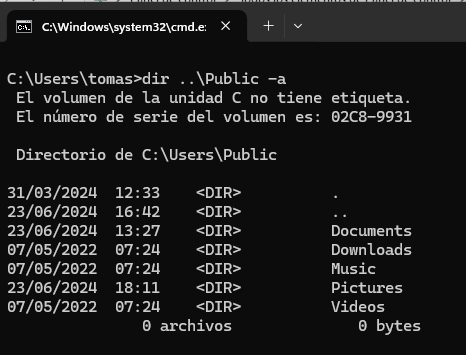
\includegraphics[width=0.75\textwidth,height=\textheight]{png/CarpetaPublic.png}
\caption{\emph{Figura 2:Carpetes públiques}}
\end{figure}

\begin{quote}
Nota: Les carpetes públiques de Windows son accessibles per als usuaris
locals (que s'autentiquen en inicair sessió, evidentment). De fet, el
seu ús principal és compartir informació entre ells.
\end{quote}

\textbf{Conclusions}

\begin{itemize}
\tightlist
\item
  Ens protegirem d'accesos maliciosos o accidental en xarxes públiques.
\item
  Coneguem la utilitat de les carpetes públiques. Podríem usar-ho en un
  WorkGroup senzill però el normal és que necessitem compartir les dades
  en altres unitats i més carpetes.
\item
  Per treballar en una xarxa local (Workgroup o Domini) com anem a fer
  en aquest mòdul, cal que el PC puga descobrir els altres dispositius i
  ser descobert per altri en la XARXA PRIVADA.
\end{itemize}

\begin{figure}
\centering
\includegraphics[width=0.75\textwidth,height=\textheight]{png/configuraciónAvanzadaDeUsoCompartido.png}
\caption{\emph{Figura 4: Configuració per a un WorkGroup i Domini}}
\end{figure}

\subsection{2.3 Canvi de Pública a Privada i ``Red No
indentificada''}\label{canvi-de-puxfablica-a-privada-i-red-no-indentificada}

Inicialment trobarem la xarxa com a \textbf{No indentificada} i no
podrem canviar-la a PRIVADA/PÚBLICA

\begin{figure}
\centering
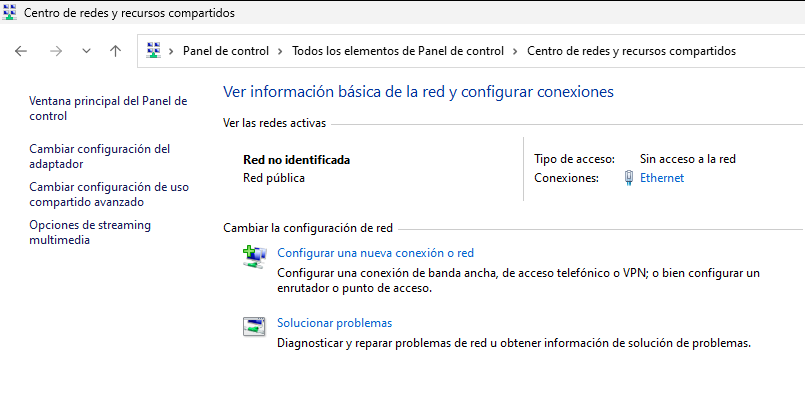
\includegraphics[width=0.75\textwidth,height=\textheight]{png/redNoIdentificada.png}
\caption{\emph{Figura 5:Red NO identificada}}
\end{figure}

Fent un poc d'spoiler al tema de Directives (és inevitable en SO), la
solució passa per\ldots{}

\begin{itemize}
\tightlist
\item
  Win + R
\item
  secpol.msc
\end{itemize}

\begin{figure}
\centering
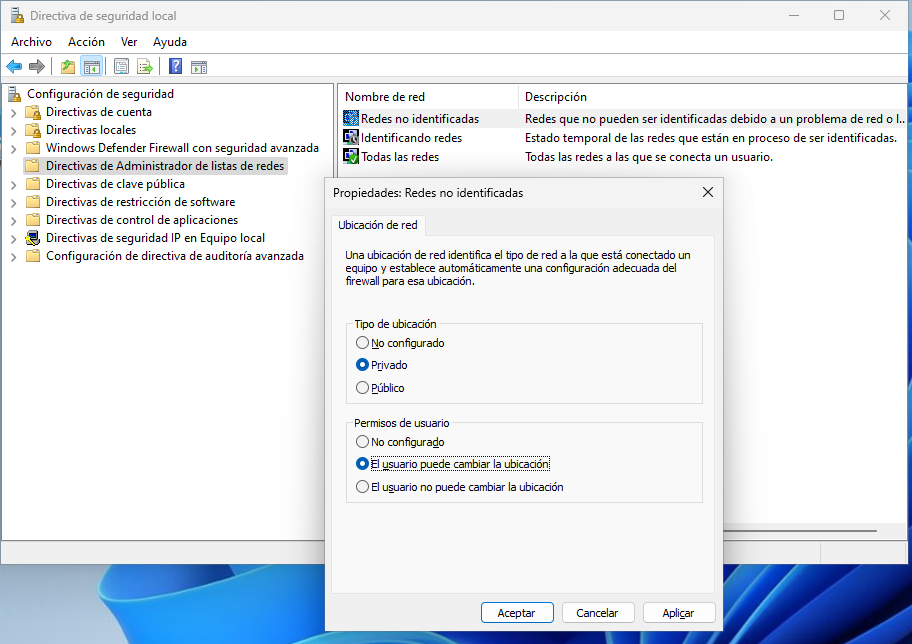
\includegraphics[width=0.75\textwidth,height=\textheight]{png/secpolRedesNoIdentificadas.png}
\caption{\emph{Figura 6:Directiva local: Redes no indentificadas}}
\end{figure}

Ho podem solucionat des de les directives locals de seguretat.

\begin{figure}
\centering
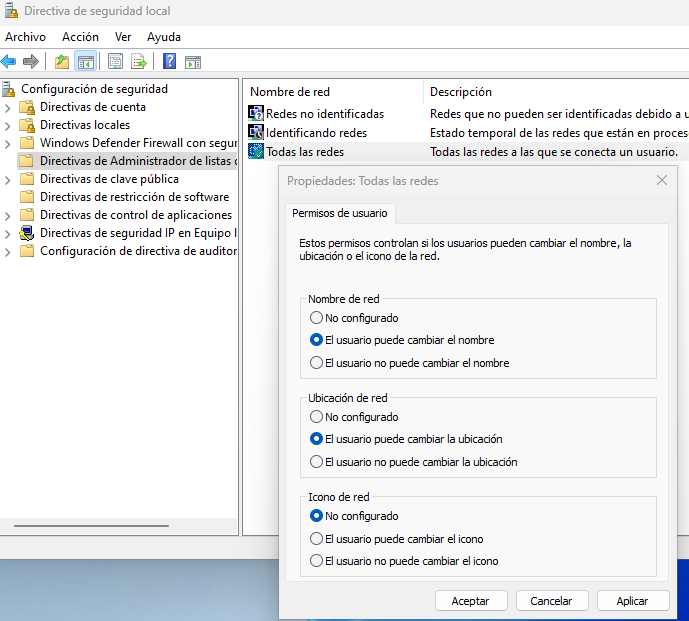
\includegraphics[width=0.75\textwidth,height=\textheight]{png/secpolRedesNoIdentificadas2.png}
\caption{\emph{Figura 7:Directiva local:Redes no indendificadas 2}}
\end{figure}

\section{3 Configuració a nivell de xarxa (Adreçament
IP)}\label{configuraciuxf3-a-nivell-de-xarxa-adreuxe7ament-ip}

Ja tenim resolta la connexió a nivell físic¹ i assegurat que el software
de sistema està configurat adientment (SO i Firewall), ara sols cal
aplicar els coneixemente d'adreçament d'IPs vistos el curs anterior en
el mòdul de XAL i assignar dos IP estàtiques privades del mateix rang.

\begin{itemize}
\tightlist
\item
  No tenim cap servidor DHCP per tant hem d'establir les IP manualment
  (estàtiques).
\item
  És un xarxa privada, evidentement.
\item
  Han de comunicar-se les màquines: el mateix rang.
\item
  En una emulació VirtualBox i ``Xarxa interna'', convé que no
  coincidisca amb el rang de la IP de l'amfitrió (DHCP del centre o del
  router de casa).
\end{itemize}

Normalment per defecte ve configurat\ldots{}

\begin{figure}
\centering
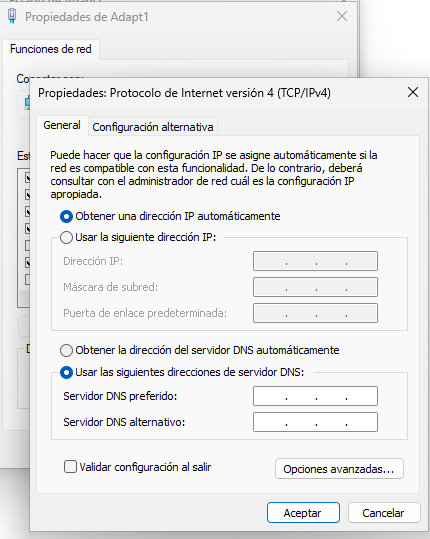
\includegraphics[width=0.75\textwidth,height=\textheight]{png/adaptador.png}
\caption{\emph{Figura 8: Adpatador DHCP}}
\end{figure}

Fem els canvis commentats:

\begin{figure}
\centering
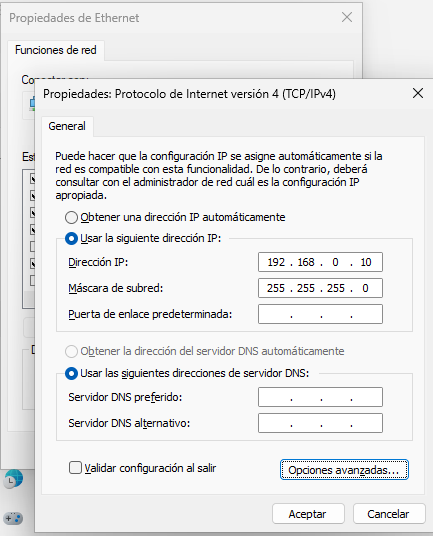
\includegraphics[width=0.75\textwidth,height=\textheight]{png/adaptador1.png}
\caption{\emph{Figura 9: Adpatador IP fixa}}
\end{figure}

\begin{figure}
\centering
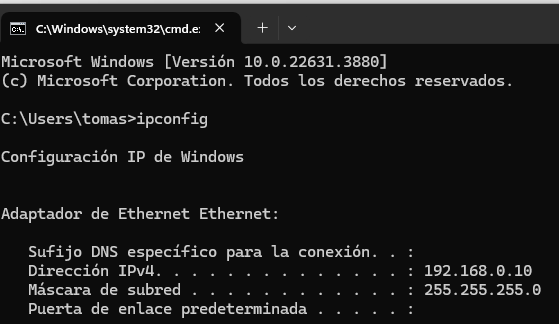
\includegraphics[width=0.75\textwidth,height=\textheight]{png/ipconfig.png}
\caption{\emph{Figura 10 Comprovem la nova IP}}
\end{figure}

¹Atenent a l'estructura ISO/OSI diríem Nivell Físic i també d'Accés al
Medi però en el nostre mòdul no cal entrar en aquests detalls.

\section{4 WORKGROUP}\label{workgroup}

Ja hem resolt els punt 1, 2 i en falta el 3.:

\begin{enumerate}
\def\labelenumi{\arabic{enumi}.}
\tightlist
\item
  Connexió física.
\item
  Restriccions de la xarxa.

  \begin{itemize}
  \tightlist
  \item
    Xarxa privada.
  \item
    Compartir arxius i impressores.
  \item
    Detecció per al xarxa.
  \item
    Firewall.
  \end{itemize}
\end{enumerate}

\section{3. Crear el Workgroup (grup de
treball).}\label{crear-el-workgroup-grup-de-treball.}

\subsection{3.1 Afegir els dos PCs al
Workgroup}\label{afegir-els-dos-pcs-al-workgroup}

Realment no hem de ``crear'' el Grup de Treball sinó que en afegir els
PC a ell ja està creat. Hem danat a Panel de
\textbf{Control\textbackslash Sistema\textbackslash Información\textbackslash Dominio
o grupo de trabajo}

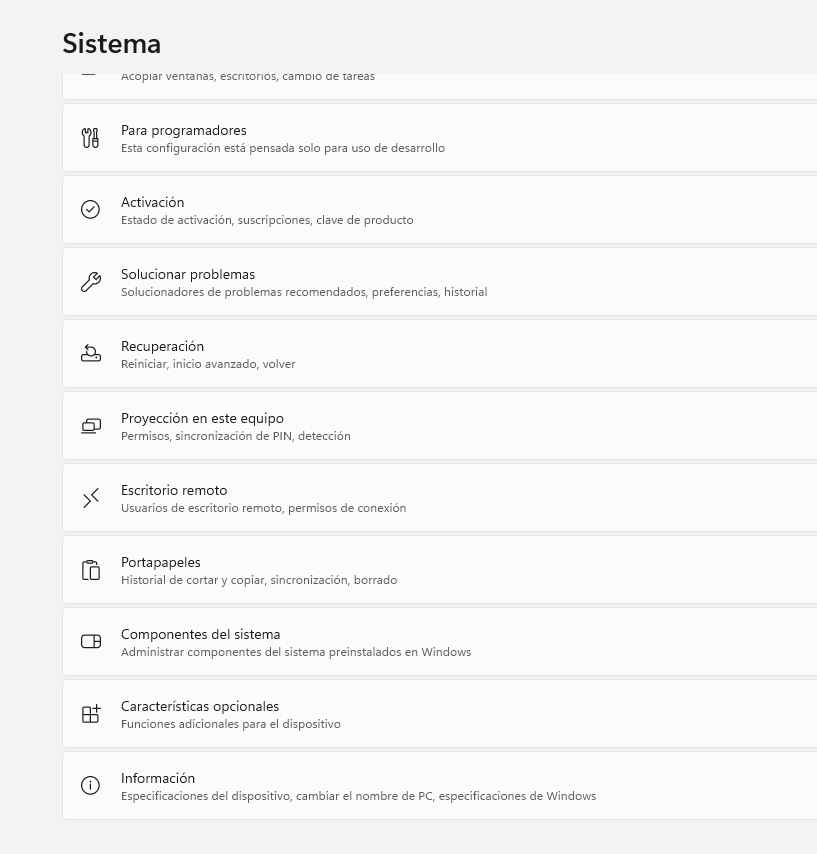
\includegraphics[width=0.75\textwidth,height=\textheight]{png/informacionSistema1.png}

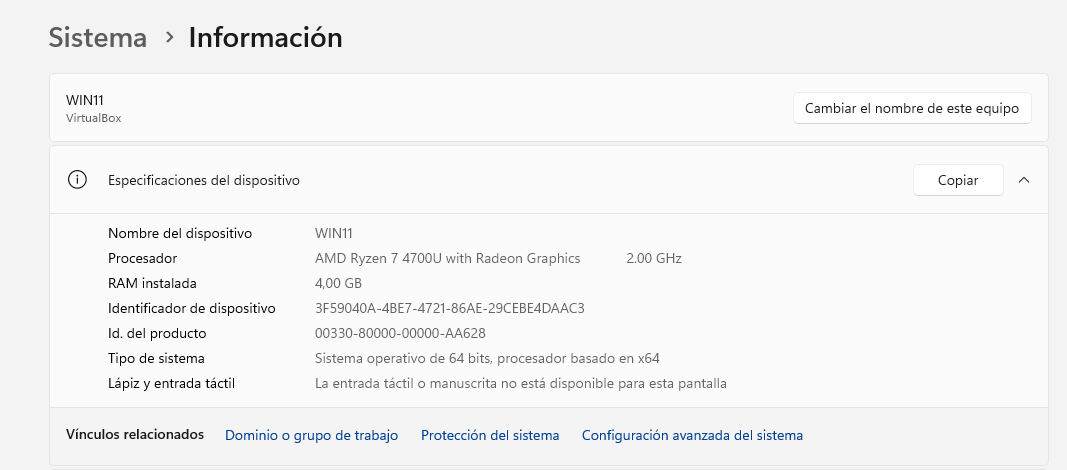
\includegraphics[width=0.75\textwidth,height=\textheight]{png/informacionSistema2.png}

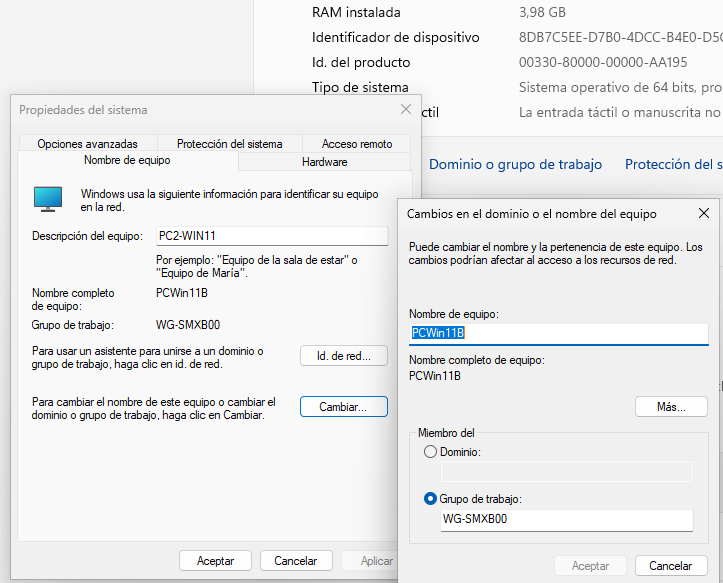
\includegraphics[width=0.75\textwidth,height=\textheight]{png/workgroup1.png}

També des de ``Mi equipo''\textbackslash propiedades.

És l'opció que ens permet canviar el nom del PC i també de:

\begin{itemize}
\tightlist
\item
  Workgrup (grup de treball)
\item
  Domini
\end{itemize}

En fer els canvis als PC i reiniciar-los haurem creat la xarxa més
senzilla. Pot ser útil per a:

\begin{itemize}
\tightlist
\item
  xicotetes organitzacions amb pocs PC o impressores.
\item
  xarxes amb poc treball col·laboratiu.
\end{itemize}

\begin{quote}
Nota: Tot i que en la literatura de SO sol identificar-se un Grup de
Treball amb una LAN amb pocs PC i un Domini amb una LAN de més de 10, 15
ó 20 PC, no necessàriament ha de ser així. Podem tindre 20 PC que usen
el núvol per a tot i molt esporàdicament comparteixen una carpeta entre
ells. També tindre només 7 PC en la LAN que usen un ERP amb la seua BD i
backup i es carpetes amb diferents permisos segons els usuaris.
\end{quote}

\subsection{3.2 Compartir un recurs}\label{compartir-un-recurs}

Comp ja vam vore el curs passat, podem compartir un recurs (carpeta) amb
permís de lectura o escritura per qualsevol usuari (\textbf{Todos}) o
anar afegint els usuaris i indicant quin tipus de permís.

Si volem restringir l'accès a determinats usuaris de la xarxa, haurem de
tindre els \textbf{usuaris ``replicats'' en cada PC} on compartim un
recurs.

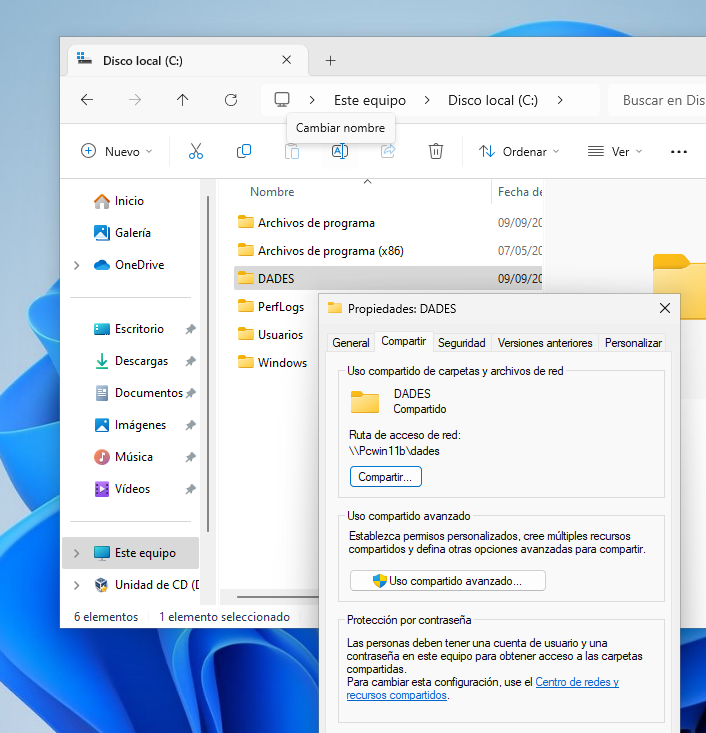
\includegraphics[width=0.75\textwidth,height=\textheight]{png/compartir1.png}

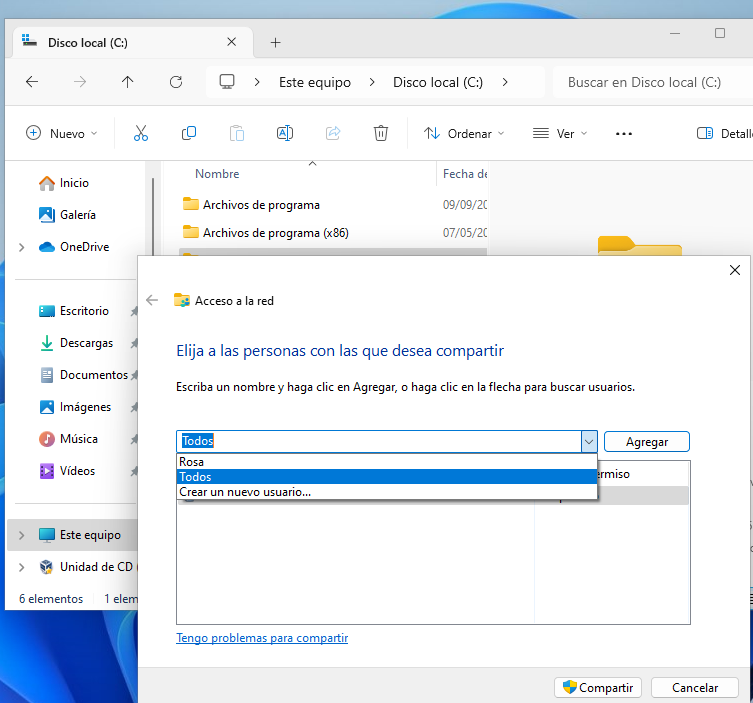
\includegraphics[width=0.75\textwidth,height=\textheight]{png/compartir2.png}

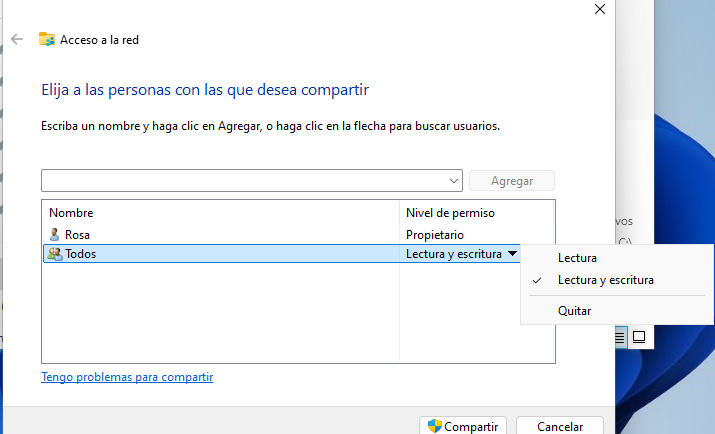
\includegraphics[width=0.75\textwidth,height=\textheight]{png/compartir3.png}

\end{document}
